\documentclass[18pt]{beamer}
\usetheme{Madrid}

\usepackage{graphics}


\newcommand{\centeredlargetext}[3]{
{
\setbeamertemplate{navigation symbols}{}
\setbeamercolor{background canvas}{bg={#1}}
\color{#2}
\begin{frame}[plain]
\fontsize{36pt}{36pt}\selectfont
\center
\begin{center}
{#3}
\end{center}
\end{frame}
}}

\newcommand{\centeredhugetext}[3]{
{
\setbeamertemplate{navigation symbols}{}
\setbeamercolor{background canvas}{bg={#1}}
\fontsize{72pt}{72pt}\selectfont
\color{#2}
\begin{frame}[plain]
\center
\begin{center}
{#3}
\end{center}
\end{frame}
}}


\begin{document}

\title[Magic Cauldron]{The Magic Cauldron}
\subtitle[]{Open Source Software Practice\\
CSCI-4967 / ECSE-4968}
\author[Ibanez]{Dr. Luis Ibanez}
\institute[Kitware]{KITWARE Inc. Clifton Park, NY}
\date[August 2012]{August 30 2012}


\begin{frame}
\titlepage
\end{frame}


{
\setbeamertemplate{navigation symbols}{}
\begin{frame}[plain]
\center
\begin{center}
This presentation is copyrighted by\\
The \textbf{Insight Software Consortium}\\
\bigskip
distributed under the\\
\textbf{Creative Commons by Attribution License 3.0}\\
\url{http://creativecommons.org/licenses/by/3.0}\\
\bigskip
Images used in this presentation are attributed in the last slide.
\end{center}
\end{frame}
}


\centeredlargetext{black}{green}{
% purposely empty
}


\section{Business Models}
{
\setbeamertemplate{navigation symbols}{}
\setbeamertemplate{background canvas}{
  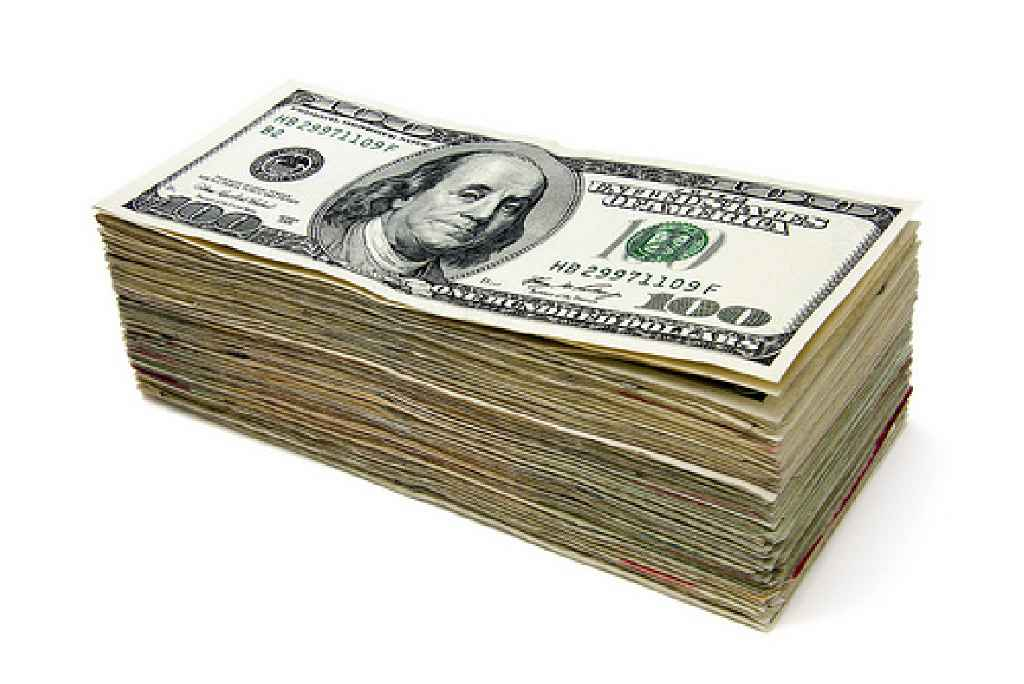
\includegraphics[width=\paperwidth,height=\paperheight]{../Art/3366720659_small.jpg}
}
\begin{frame}[plain]
\end{frame}
}


\centeredlargetext{black}{white}{
Can I make money\\
writing\\
Open Source software ?
}


\centeredhugetext{black}{white}{
Yes~!
}


\centeredhugetext{black}{white}{
10
}


\centeredhugetext{black}{white}{
\$
}


\centeredhugetext{black}{white}{
85\%~\pause~Ms.
}


\centeredhugetext{black}{white}{
42\%~\pause~Ph.D.
}


\centeredhugetext{black}{white}{
\$~~:-)
}


\centeredhugetext{black}{white}{
C[\_\_]
}


\centeredhugetext{black}{white}{
HW~\pause~\$3K
}


\centeredhugetext{black}{white}{
Hack, Hack !\ldots
}


\centeredhugetext{black}{white}{
git push
}


\centeredhugetext{black}{white}{
FREE~!
}


\centeredhugetext{black}{white}{
2~\pause~1998
}


\centeredhugetext{black}{white}{
105~\pause~2012
}


\centeredhugetext{black}{white}{
$e^x$~\pause~14 years
}


\centeredhugetext{black}{white}{
64\%~\pause~2011
}


\centeredhugetext{black}{white}{
50\%~Annual
}


\centeredhugetext{black}{white}{
\$27.2M~\pause~2011
}


\centeredhugetext{black}{white}{
E+=48\pause\\
Since 2009
}


\centeredhugetext{black}{white}{
248\%\\
3-year Growth
}

\centeredlargetext{black}{white}{
Rank \#100\\
\pause
Fastest Growing\\
Software Company
}

\centeredlargetext{black}{white}{
Rank \#1245\\
\pause
Fastest Growing\\
Company
}


\centeredhugetext{black}{white}{
Debt~\pause$=$~\$0
}


\centeredhugetext{black}{white}{
Profitable\\
\pause
every year
}


\centeredhugetext{black}{white}{
It Works !
}


\centeredhugetext{black}{white}{
Fastest Growing\\
Software Company ?
}


\centeredhugetext{black}{white}{
Acquia
}


\centeredhugetext{black}{white}{
Drupal\\
Services
}


\centeredhugetext{black}{green}{
\ldots
}


\section{Manufacturing Delusion}


\centeredlargetext{black}{green}{
\emph{Let me tell you\\
\bigskip
why you are here\ldots}
}


\centeredlargetext{black}{green}{
\emph{You are here\\
\bigskip
because\\
\bigskip
You know something\ldots
}
}


\centeredlargetext{black}{green}{
\emph{What you know\\
\bigskip
you can't explain\ldots
}
}


\centeredlargetext{black}{green}{
\emph{but you feel it\ldots
}
}


\centeredlargetext{black}{green}{
\emph{You felt it\\
\bigskip
your entire life\ldots
}
}


\centeredlargetext{black}{green}{
\emph{That there is\\
\bigskip
someting wrong\\
\bigskip
with the world\\
\bigskip
you don't know\\
\bigskip
what it is\ldots
\bigskip
}
}


\centeredlargetext{black}{green}{
\emph{but it's there\ldots
}
}


\centeredlargetext{black}{green}{
\emph{like a splinter\\
\bigskip
in your mind\ldots
\bigskip
}
}


\centeredlargetext{black}{green}{
\emph{driving you mad\ldots
}
}


\centeredlargetext{black}{green}{
\emph{It is this feeling\\
\bigskip
that has brought\\
\bigskip
you to me\ldots
}
}


\centeredlargetext{black}{green}{
\emph{Do you know\\
\bigskip
what I'm talking\\
\bigskip
about ?\ldots
}
}


\centeredlargetext{black}{green}{
\emph{The Matrix ?
}
}


\centeredlargetext{black}{green}{
\emph{Do you want\\
\bigskip
to know\\
\bigskip
what it is ?\ldots
}
}



\centeredlargetext{black}{green}{
\emph{It is the world\\
\bigskip
that has been pulled\\
\bigskip
over your eyes\ldots
}
}



\centeredlargetext{black}{green}{
\emph{To blind you\\
\bigskip
from the truth\ldots
}
}


\centeredlargetext{black}{green}{
\emph{What truth ?
}
}


\centeredlargetext{black}{green}{
The Software\\
Manufacturing\\
Delusion
}

{
\setbeamertemplate{navigation symbols}{}
\setbeamercolor{background canvas}{bg=black}
\color{white}
\begin{frame}[plain]
\fontsize{18pt}{18pt}\selectfont
\color{white}
\emph{
Software is largely a \textbf{service} industry\\
\pause
operating under the persistent\\
\pause
but unfounded \textbf{delusion}\\
\pause
that it is a \textbf{manufacturing} industry.
}
\pause
\bigskip
\begin{flushright}
Eric S. Raymond
\end{flushright}
\end{frame}
}


{
\setbeamertemplate{navigation symbols}{}
\setbeamertemplate{background canvas}{
  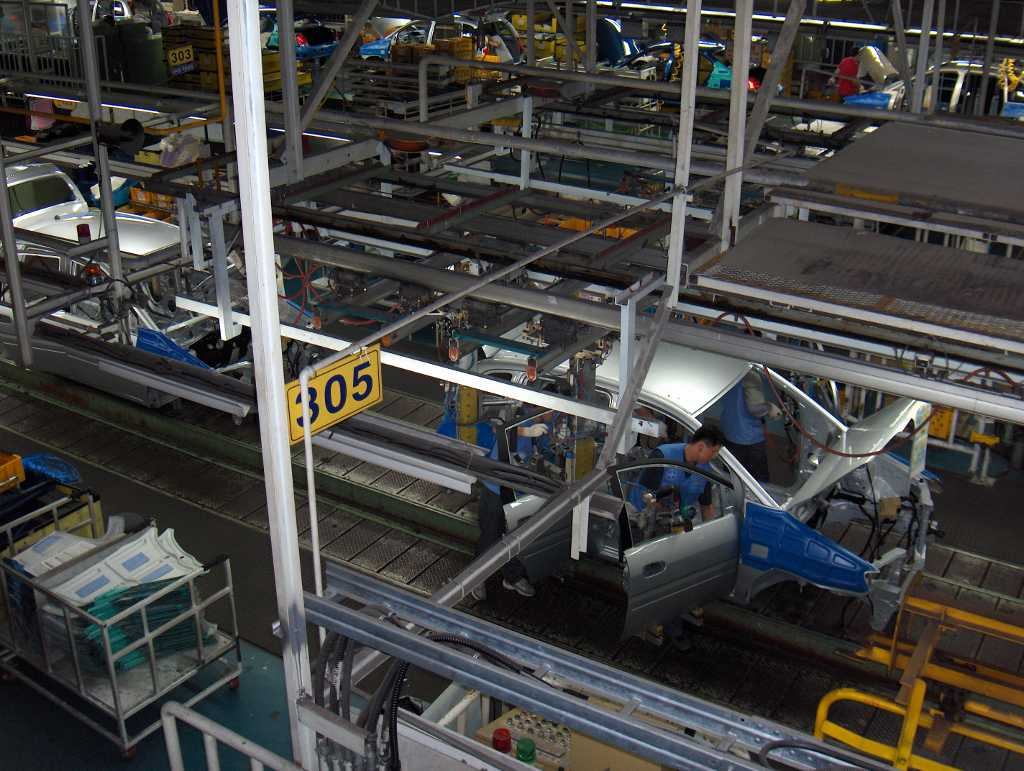
\includegraphics[width=\paperwidth,height=\paperheight]{../Art/Hyundai_car_assembly_line_scaled.jpg}
}
\begin{frame}[plain]
\end{frame}
}


\begin{frame}
\frametitle{Manufacturing Business Model}
\Huge
\begin{itemize}
\item Come up with an Idea
\pause
\item Raise capital
\pause
\item Hire workers
\pause
\item Manufacture items
\pause
\item Do Marketing
\pause
\item Sell Units
\end{itemize}
\end{frame}


\section{Software as Product}


{
\setbeamertemplate{navigation symbols}{}
\begin{frame}
\frametitle{Disguising Software as a Product}
\begin{center}
  
\includegraphics[width=0.4\paperwidth,height=0.8\paperheight]{../Art/4047547668_f46315f196_smaller.jpg}
  
\includegraphics[width=0.4\paperwidth,height=0.8\paperheight]{../Art/4047547668_f46315f196_smaller.jpg}
\end{center}
\end{frame}
}


{
\setbeamertemplate{navigation symbols}{}
\setbeamertemplate{background canvas}{
  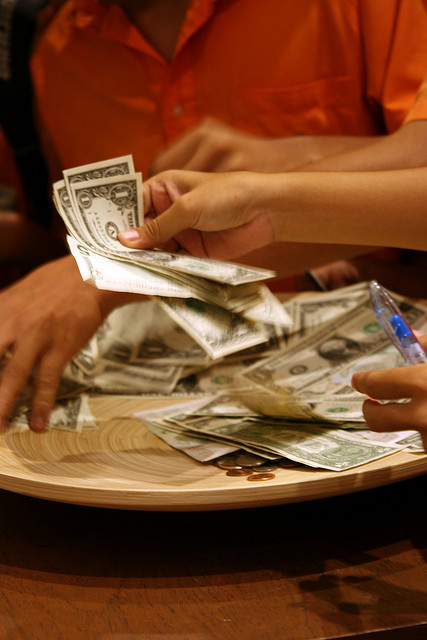
\includegraphics[width=0.55\textwidth,height=\paperheight]{../Art/2672465894_5b21e12135_z.jpg}
  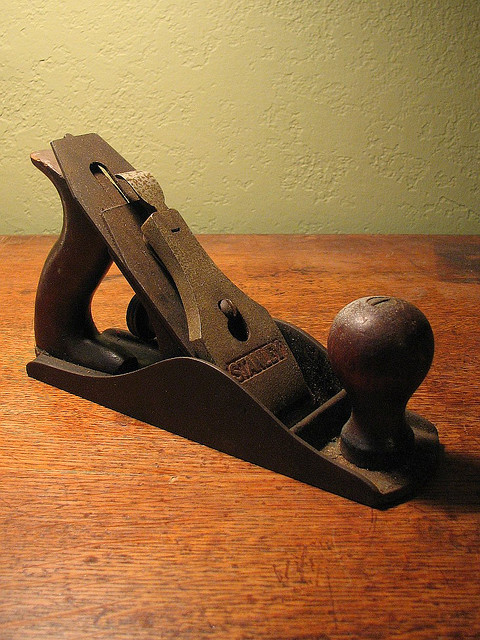
\includegraphics[width=0.55\textwidth,height=\paperheight]{../Art/4293485922_7474ef04ce_z.jpg}
  }
\begin{frame}
\frametitle{Sale Value vs Use Value}
\end{frame}
}


\centeredlargetext{black}{white}{
Licensed !\\
\bigskip
\pause
Not Sold\ldots
}


\subsection{Largest Software Publishers}


\centeredlargetext{black}{white}{
The Largest\\
\bigskip
\pause
Software Publishers
}


\centeredhugetext{black}{white}{
2011
}


{
\setbeamertemplate{navigation symbols}{}
\begin{frame}
\frametitle{Largest Software Publishers - 2011}

\begin{center}
\begin{tabular}{clrrr}
\hline
  \textbf{Rank
\footnote{
\url{http://www.softwaretop100.org/global-software-top-100-edition-2011}}
} &\textbf{Publisher} & \textbf{Software \$M} & \textbf{Total \$M} & \textbf{Percent} \\
\hline
\hline
1 &  \textbf{Microsoft} & 54,270 & 67,383 & 80.5\% \\
2 &  \textbf{IBM} & 22,485 & 99,870 & 22.5\% \\
3 &  \textbf{Oracle} & 20,958 & 30,180 & 69.4\% \\
4 &  SAP & 12,558 & 16,654 & 75.4\% \\
5 &  Ericsson & 7,274 & 30,307 & 24.0\% \\
6 &  HP & 6,669 & 126,562 & 5.3\% \\
7 &  \textbf{Symantec} & 5,636 & 6,013 & 93.7\% \\
8 &  Nintendo & 5,456 & 13,766 & 39.6\% \\
9 &  Blizzard & 4,447 & 4,447 & 100.0\% \\
10&  EMC & 4,356 & 17,015 & 25.6\% \\
\end{tabular}

\end{center}
\end{frame}
}


{
\setbeamertemplate{navigation symbols}{}
\begin{frame}
\frametitle{Largest Software Publishers - 2011}

\begin{center}
\begin{tabular}{clrrr}
\hline
  \textbf{Rank
\footnote{
\url{http://www.softwaretop100.org/global-software-top-100-edition-2011}}
} &\textbf{Publisher} & \textbf{Software \$M} & \textbf{Total \$M} & \textbf{Percent} \\
\hline
\hline
11 & \textbf{Nokia Siemens} & 4,229 & 16,918 & 25.0\% \\
12 & CA & 4,136 & 4,454 & 92.9\% \\
13 & Electronic Arts & 3,413 & 3,413 & 100.0\% \\
14 & \textbf{Adobe} & 3,177 & 3,826 & 83.0\% \\
15 & Alcatel-Lucent & 2,561 & 21,374 & 12.0\% \\
16 & Cisco & 2,383 & 41,045 & 5.8\% \\
17 & Sony & 2,083 & 83,039 & 2.5\% \\
18 & Hitachi & 1,939 & 113,500 & 1.7\\% \\
19 & Dassault & 1,885 & 2,090 & 90.2\% \\
20 & BMC & 1,843 & 1,981 & 93.0\% \\
\end{tabular}

\end{center}
\end{frame}
}




{
\setbeamertemplate{navigation symbols}{}
\begin{frame}
\frametitle{Largest Software Publishers - 2011}

\begin{center}
\begin{tabular}{clrrr}
\hline
  \textbf{Rank
\footnote{
\url{http://www.softwaretop100.org/global-software-top-100-edition-2011}}
} &\textbf{Publisher} & \textbf{Software \$M} & \textbf{Total \$M} & \textbf{Percent} \\
\hline
\hline
21 & SunGard & 1,762 & 4,992 & 35.3\%  \\
22 & \textbf{Autodesk} & 1,701 & 1,932 & 88.0\%  \\
23 & Konami & 1,643 & 3,122 & 52.6\%   \\
24 & Salesforce.com & 1,523 & 1,628 & 93.6\% \\
25 & Sage & 1,485 & 2,228 & 66.7\%  \\
26 & Ubisoft & 1,441 & 1,441 & 100.0\%  \\
27 & \textbf{VMWare} & 1,399 & 2,851 & 49.1\%  \\
28 & \textbf{Apple} & 1,358 & 75,660 & 1.8\%  \\
29 & Infor & 1,350 & 1,800 & 75.0\%  \\
30 & Intuit & 1,326 & 3,133 & 42.3\%  \\
\end{tabular}

\end{center}
\end{frame}
}


\centeredhugetext{black}{white}{
2010
}


{
\setbeamertemplate{navigation symbols}{}
\begin{frame}
\frametitle{Largest Software Publishers - 2010}

\begin{center}
\begin{tabular}{clrrr}
\hline
  \textbf{Rank
\footnote{
\url{http://www.softwaretop100.org/global-software-top-100-edition-2010}}
} &\textbf{Publisher} & \textbf{Software \$M} & \textbf{Total \$M} & \textbf{Percent} \\
\hline
\hline
1 &  \textbf{Microsoft} & 49,090  & 61,159 &  80\% \\
2 &  \textbf{IBM} & 21,396  & 95,758  & 22\% \\
3 &  \textbf{Oracle} & 18,582  & 22,734 &  82\% \\
4 &  SAP & 11,368  & 15,373 &  74\% \\
5 &  Ericsson & 7,595  & 29,014 &  26\% \\
6 &  Nintendo & 6,799  &  17,762 &  38\% \\
7 &  HP & 6,183  &  116,245 &  5\% \\
8 &  \textbf{Symantec} & 5,565  & 5,992 &  93\% \\
9 &  Nokia Siemens & 4,529  &  18,114 &  25\% \\
10&  Blizzard & 4,279  & 4,279 & 100\% \\
\end{tabular}

\end{center}
\end{frame}
}


{
\setbeamertemplate{navigation symbols}{}
\begin{frame}
\frametitle{Largest Software Publishers - 2010}

\begin{center}
\begin{tabular}{clrrr}
\hline
\textbf{Rank
\footnote{
\url{http://www.softwaretop100.org/global-software-top-100-edition-2010}}
} &\textbf{Publisher} & \textbf{Software \$M} & \textbf{Total \$M} & \textbf{Percent} \\
\hline
\hline
11 & CA & 4,012  & 4,318 & 93\% \\
12 & EMC & 3,960  & 14,026 & 28\% \\
13 & \textbf{Electronic Arts} & 3,728  &  3,728 & 100\% \\
14 & \textbf{Adobe} & 2,796 &  2,987 & 94\% \\
15 & Cisco & 2,137 & 36,633 & 6\% \\
16 & SunGard & 1,996  & 5,508 & 36\% \\
17 & Sony & 1,914 &  79,441 & 2\% \\
18 & BMC & 1,758& 1,888 & 93\% \\
19 & Alcatel-Lucent & 1,635  &  21,835 & 8\% \\
20 & Konami & 1,594 &  2,887 & 55\% \\
\end{tabular}

\end{center}
\end{frame}
}


{
\setbeamertemplate{navigation symbols}{}
\begin{frame}
\frametitle{Largest Software Publishers - 2010}

\begin{center}
\begin{tabular}{clrrr}
\hline
\textbf{Rank
\footnote{
\url{http://www.softwaretop100.org/global-software-top-100-edition-2010}}
} &\textbf{Publisher} & \textbf{Software \$M} & \textbf{Total \$M} & \textbf{Percent} \\
\hline
\hline
21 & Hitachi & 1,589 & 99,818 & 2\% \\
22 & Dassault & 1,584 & 1,803 & 88\% \\
23 & Infor & 1,575 & 2,100 & 75\% \\
24 & Sage & 1,557 & 2,336 & 67\% \\
25 & \textbf{Autodesk} & 1,557 & 1,764 & 88\% \\
\ldots & \ldots & \ldots & \ldots & \ldots \\
28 & \textbf{Apple} & 1,218 & 43,086 &  \textbf{3\%}  \\
32 & SAS Institute & 1,155  &  2,310 & 50\%  \\
37 & VMWare & 1,029 & 2,024 &  51\%  \\
39 & McAfee & 964 & 1,927 & 50\% \\
\end{tabular}

\end{center}
\end{frame}
}


\begin{frame}
\frametitle{Distribution of Software Publisher Size}
  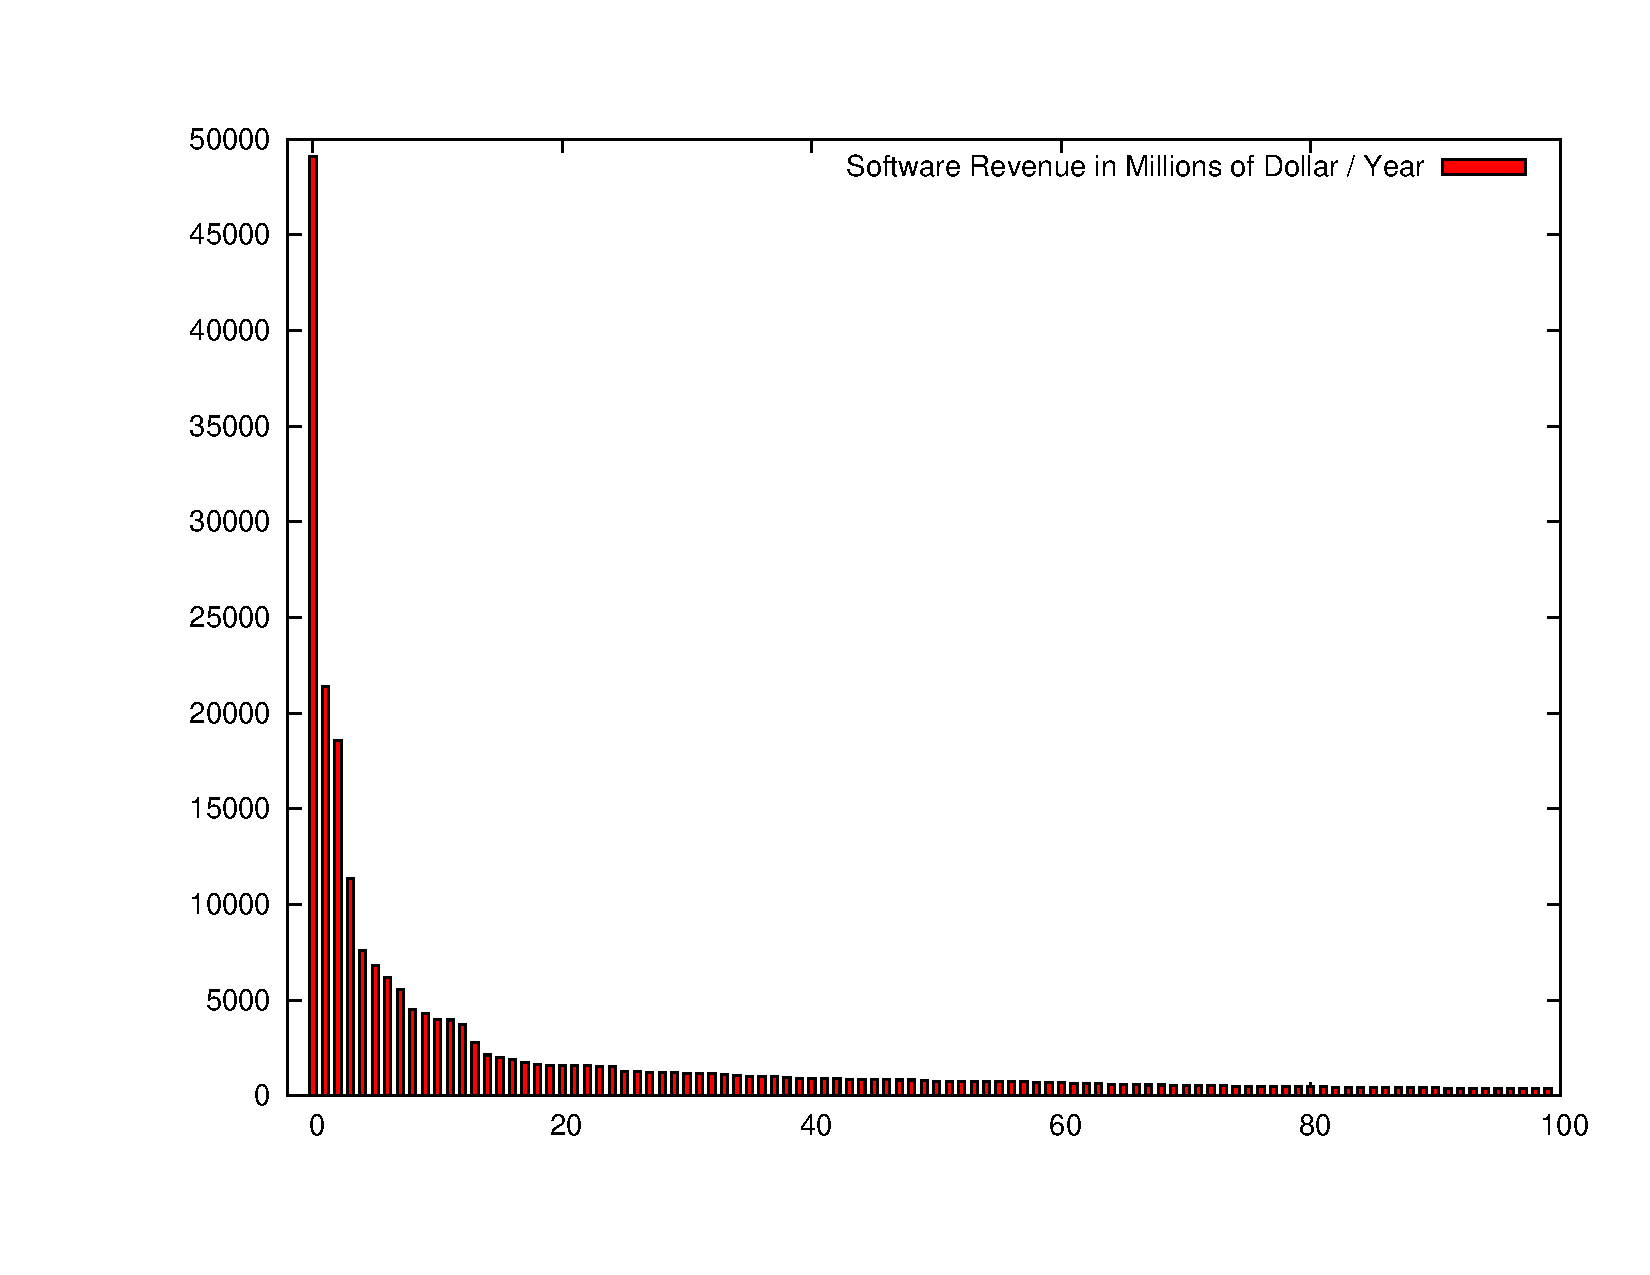
\includegraphics[width=0.9\textwidth,height=0.9\paperheight]{../Art/LargestSoftwarePublishersPlot.pdf}
\end{frame}


\begin{frame}
\frametitle{Size of the Software Publishing Industry - 2010}
\fontsize{72pt}{90pt}\selectfont
\begin{center}
\$ 221 Billion
\end{center}
\end{frame}


\begin{frame}
\frametitle{Some Notable Companies}
\begin{tabular}{lrrr}
\hline
\textbf{Publisher} & \textbf{Annual Revenue} & \textbf{Cost of Revenue} & \textbf{Gross Profit} \\
\hline
\hline
\href{http://www.google.com/finance?fstype=ii\&q=NASDAQ:MSFT}{Microsoft Corp.} & \$ 62,484 M & \$ 12,395 M  & \$ 50,089 M  \\
\hline
\href{http://www.google.com/finance?q=NYSE:IBM\&fstype=ii}{IBM Corp.} & \$ 95,759 M & \$ 51,972 M & \$ 43,787 M \\
\hline
\href{http://www.google.com/finance?q=NASDAQ:AAPL\&fstype=ii}{Apple Inc.} & \$ 42,905 M & \$ 25,683 M & \$ 17,222 M \\
\hline
\href{http://www.google.com/finance?q=NASDAQ:ORCL\&fstype=ii}{Oracle} & \$ 26,820 M & \$ 5,764 M & \$ 21,056 M \\
\hline
\href{http://www.google.com/finance?q=NASDAQ:SYMC\&fstype=ii}{Symantec} & \$ 5,985 M & \$ 1,105 M & \$ 4,880 M \\
\hline
\href{http://www.google.com/finance?q=NASDAQ:ADBE\&fstype=ii}{Adobe} & \$ 943 M & \$ 107 M & \$ 835 M \\
\hline
\end{tabular}
\bigskip
\begin{center}
Balance Sheets - September 2009 - September 2010
\end{center}
\end{frame}


{
\setbeamertemplate{navigation symbols}{}
\begin{frame}
\frametitle{IBM- 2011}
\begin{center}
\begin{tabular}{lrr}
\hline
\textbf{Product}
\footnote{IBM 2011 Financial Report (page 27):
\url{http://www.ibm.com/annualreport/2011/bin/assets/2011_ibm_annual.pdf}}
& \textbf{Revenue Percent} \\
\hline
\hline
Global Technology Services & 38.5\% \\
Global Business Services & 18.2\% \\
\textbf{Software} & \textbf{23.5\%}\\
Systems and Technology & 17.9\% \\
Global Financing & 2.0\% \\
\hline
\end{tabular}
\end{center}
\end{frame}
}


{
\setbeamertemplate{navigation symbols}{}
\begin{frame}
\frametitle{Apple Inc. - 2011}

\begin{center}
\begin{tabular}{lrr}
\hline
\textbf{Product}
\footnote{
\href{http://phx.corporate-ir.net/External.File?item=UGFyZW50SUQ9NzgwODJ8Q2hpbGRJRD0tMXxUeXBlPTM=&t=1}
{Financial Report, 1st Quarter 2011, page 25:}
 \url{http://www.apple.com/investor/} }
& \textbf{Sales \$M}
& \textbf{Percent} \\
\hline
\hline
\textbf{iPhone} and services & 10,468 & \textbf{39.15\%}  \\
iPad and services & 4,608 & 17.23\% \\
Laptops & 3,699 & 13.83\% \\
iPod & 3,425 & 12.81\% \\
Desktops & 1,731 & 6.47\% \\
Music and services & 1,431 & 5.35\%  \\
\textbf{Software} and others &  786 & \textbf{2.94\%} \\
Perihelias &  593 & 2.22\% \\
\hline
Total &  26,741 & 100\% \\
\end{tabular}

\end{center}
\end{frame}
}


{
\setbeamertemplate{navigation symbols}{}
\begin{frame}
\frametitle{Apple Inc. - 2012}

\begin{center}
\begin{tabular}{lrr}
\hline
\textbf{Product}
\footnote{
\href{http://files.shareholder.com/downloads/AAPL/2036902658x0x585701/beacb369-cb95-4950-acf4-4fbfa3569ec6/Q3\_2012\_Form\_10-Q\_As-Filed\_.pdf}
{Financial Report, 3rd Quarter 2012, page 26:}
 \url{http://www.apple.com/investor/} }
& \textbf{Sales \$M}
& \textbf{Percent} \\
\hline
\hline
\textbf{iPhone} and services & 16,245 &  \textbf{46.38\%}  \\
iPad and services & 9,171 & 26.19\% \\
Laptops & 3,646 & 10.41\% \\
iPod & 1,060 & 3.03\% \\
Desktops & 1,287 & 3.67\% \\
Music and services & 2,060 & 5.88\%  \\
\textbf{Software} and others &  891 & \textbf{2.54\%} \\
Perihelias &  663 & 1.89\% \\
\hline
Total &  35,023 & 100\% \\
\end{tabular}

\end{center}
\end{frame}
}


\centeredlargetext{black}{white}{
How big\\
\bigskip
\pause
is the\\
\bigskip
\pause
\textbf{Software for Use}\\
\bigskip
\pause
Industry ?\ldots
}


\centeredlargetext{black}{white}{
Software used\\
\bigskip
\pause
to \textbf{run}\\
\bigskip
\pause
an institution\\
}


\centeredlargetext{black}{white}{
Countries spend\\
\bigskip
\pause
6.4\% of GDP\\
\bigskip
\pause
on Information Technology
%\footnote{\url{http://simplearchitectures.blogspot.com/2009/09/cost-of-it-failure.html}}
}


\centeredlargetext{black}{white}{
43\% of which\\
\bigskip
\pause
is spent on\\
\bigskip
\pause
hardware, software and services
}


\centeredlargetext{white}{black}{
Global GDP\\
\bigskip
\pause
\$ \textbf{69 Trillion}
}


\centeredlargetext{white}{black}{
Global IT expenditures\\
\bigskip
\pause
\$ \textbf{1,897} Billion
}


\centeredlargetext{black}{white}{
but that includes\\
\bigskip
\pause
Hardware\ldots
}


\centeredlargetext{black}{white}{
The Largest\\
\bigskip
\pause
Hardware Vendors\\
}


\subsection{Largest Software Publishers}

{
\setbeamertemplate{navigation symbols}{}
\begin{frame}
\frametitle{Largest Hardware Vendors - 2009}

\begin{center}
\begin{tabular}{clrrr}
\hline
  \textbf{Rank
\footnote{
\url{http://www.hardwaretop100.org/hardware-top-100-the-world-s-largest-hardware-companies.php}}
} &\textbf{Vendor} & \textbf{Hardware Revenue \$B} & \textbf{Percent of Industry} \\
\hline
\hline
1 &  \textbf{HP} & 85.39 &  17.45\% \\
2 &  \textbf{Samsung} & 74.76 & 15.28\% \\
3 &  \textbf{Foxconn} & 61.80 &  12.63\% \\
4 &  Nokia & 46.41 & 9.48\% \\
5 &  Dell & 44.87 & 9.17\% \\
6 &  Toshiba & 44.24 &  9.04\% \\
7 &  Intel & 36.32 &  7.42\% \\
8 &  LG & 33.42 & 6.83\% \\
9 &  Cisco & 32.84 &  6.71\% \\
10&  Canon & 29.29 & 5.99\% \\
\end{tabular}

\end{center}
\end{frame}
}

{
\setbeamertemplate{navigation symbols}{}
\begin{frame}
\frametitle{Largest Hardware Vendors - 2010}

\begin{center}
\begin{tabular}{clrrr}
\hline
  \textbf{Rank
\footnote{
\url{http://www.hardwaretop100.org/hardware-companies-top-100-2010-edition.php}}
} &\textbf{Vendor} & \textbf{Hardware Revenue \$B} & \textbf{Percent of Industry} \\
\hline
\hline
1 &  \textbf{Samsung} & 77.86 & 15.28\% \\
2 &  \textbf{HP} & 73.72 &  17.45\% \\
3 &  \textbf{Foxconn} & 44.41 &  12.63\% \\
4 &  LG & 42.03 & 6.83\% \\
5 &  Nokia & 40.10 & 9.48\% \\
6 &  Toshiba & 40.06 &  9.04\% \\
7 &  Dell & 38.39 & 9.17\% \\
8 &  Intel & 34.03 &  7.42\% \\
9 &  Apple & 31.77 & 9.17\% \\
10 &  Cisco & 29.51 &  6.71\% \\
\end{tabular}

\end{center}
\end{frame}
}
\begin{frame}
\frametitle{Distribution of Harware Vendor Size}
  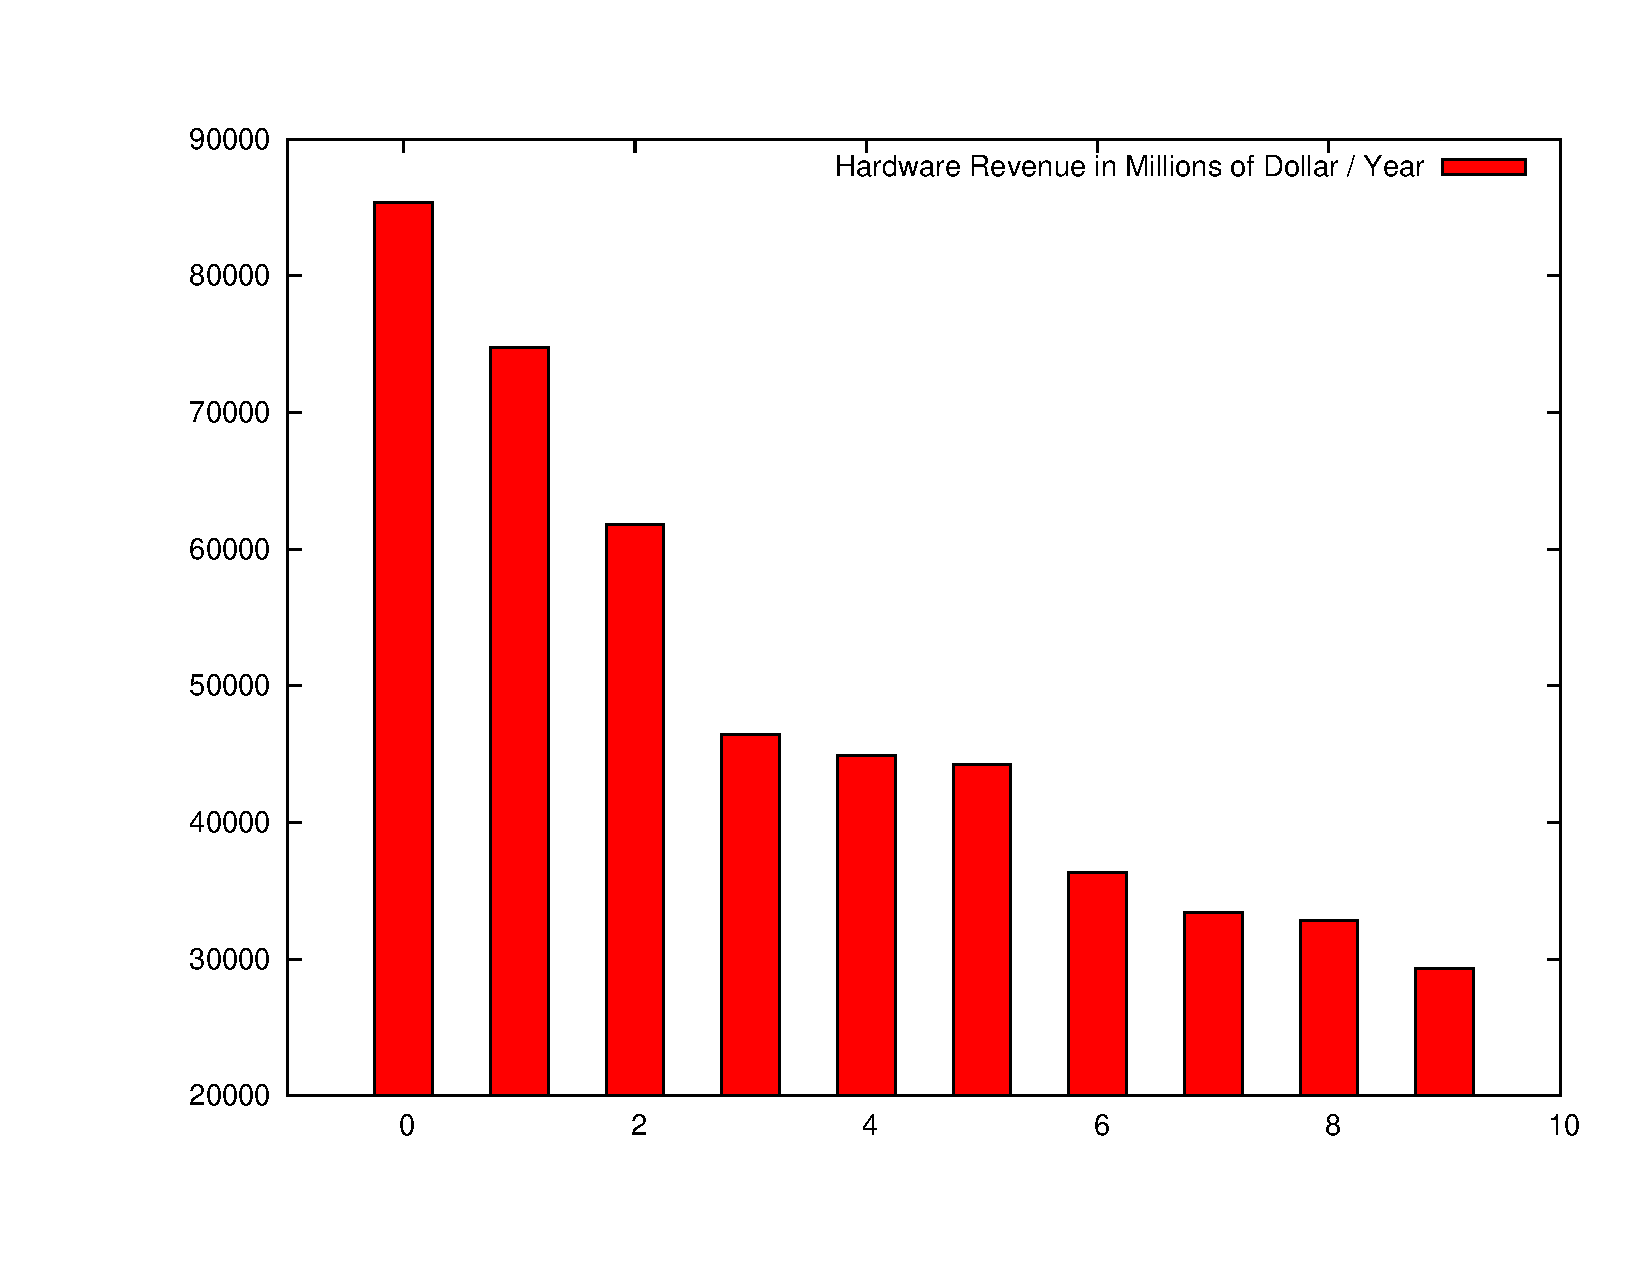
\includegraphics[width=0.9\textwidth,height=0.9\paperheight]{../Art/LargestHardwareVendorsPlot.pdf}
\end{frame}


\centeredlargetext{white}{black}{
Global\\
\bigskip
\pause
Hardware Industry\\
\bigskip
\pause
\$ \textbf{489} Billion
}


\centeredlargetext{white}{black}{
\$1,897 $-$ \$489\\
\bigskip
\pause
$=$ \\
\bigskip
\pause
\$ 1,408 Billion\\
}


\centeredlargetext{white}{black}{
Software for Sale\\
\bigskip
\pause
$:$ \\
\bigskip
\pause
Software for Use
}


\centeredlargetext{white}{black}{
\$221 B / \$1,408\\
\bigskip
\pause
$=$ \\
\bigskip
\pause
15.6\% \\
}


\centeredhugetext{black}{green}{
\ldots
}


\centeredlargetext{black}{white}{
from this\\
\bigskip
\pause
\$ 1,408 Billion\\
}



\centeredhugetext{black}{green}{
70\%~\pause~Fail !
}


\centeredhugetext{black}{green}{
\$~\text{985 B} lost
}


\centeredhugetext{black}{green}{
Every year\ldots
}


\section{Software Quality}

{
\setbeamertemplate{navigation symbols}{}
\begin{frame}
\frametitle{Lack of Quality Control}
\center
\Huge
Inadequate\\
Software Testing Infrastructure\\
costs the U.S.
\pause
\Huge
\bigskip
\begin{center}
\textbf{\$ 60 Billion} a year\footnote{\url{http://www.nist.gov/director/prog-ofc/report02-3.pdf}}
\end{center}
\end{frame}
}


{
\setbeamertemplate{navigation symbols}{}
\begin{frame}
\frametitle{Lack of Quality Control}
\Huge
\begin{center}
\textbf{\$ 0.2\%} of GDP
\end{center}
\end{frame}
}


{
\setbeamertemplate{navigation symbols}{}
\begin{frame}
\frametitle{Lack of Quality Control}
\Huge
\begin{center}
\textbf{Twice the NIH Budget}
\end{center}
\end{frame}
}


\centeredlargetext{black}{white}{
Who can save us ?
}


{
\setbeamertemplate{navigation symbols}{}
\setbeamertemplate{background canvas}{
  
\includegraphics[width=\paperwidth,height=\paperheight]{../Art/OSI_logo.png}
}
\begin{frame}[plain]
\end{frame}
}


\centeredlargetext{black}{white}{
The Tragedy\\
of the\\
Commons\\
}


\begin{frame}
\frametitle{The Tragedy of the Commons}
\Huge
\begin{itemize}
\item \textbf{Multiple} Individuals
\pause
\item Acting \textbf{Rationaly}
\pause
\item Driven by \textbf{Self-Interest}
\pause
\item Sharing a \textbf{common} resource
\end{itemize}
\end{frame}


{
\setbeamertemplate{navigation symbols}{}
\setbeamertemplate{background canvas}{
  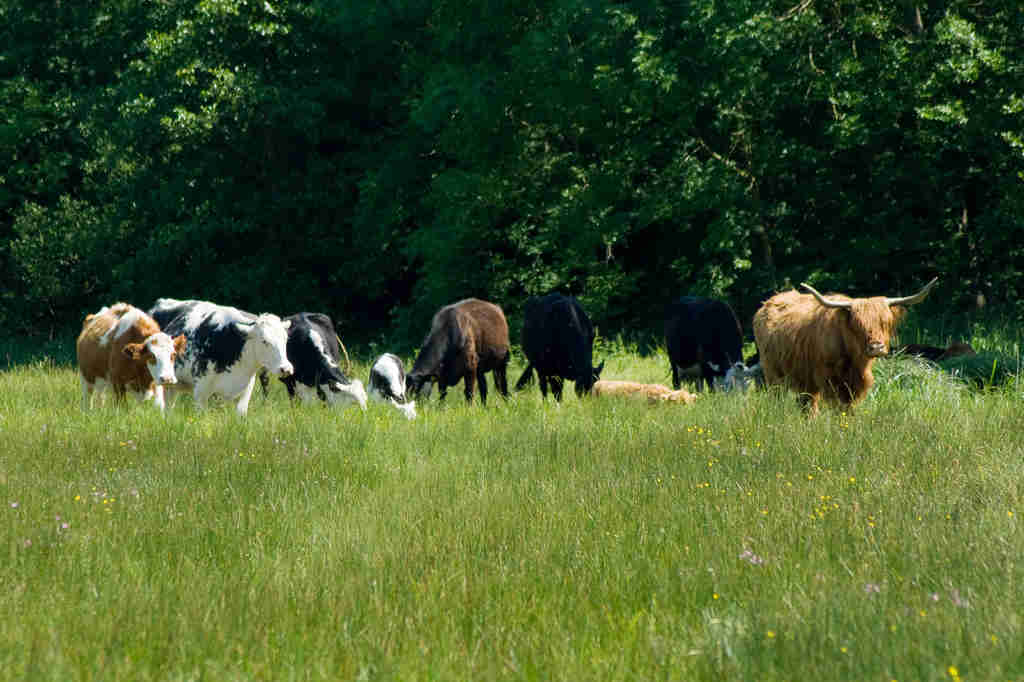
\includegraphics[width=\paperwidth,height=\paperheight]{../Art/4924182750_f128706196_b_smaller.jpg}
}
\begin{frame}[plain]
\end{frame}
}


\centeredlargetext{black}{white}{
Over-Exploitation\\
Problem
}


\centeredlargetext{black}{white}{
Under-Provision\\
Problem
}


\begin{frame}
\frametitle{The Tragedy of the Commons - Ambiguity}
\Huge
\begin{itemize}
\item Common Property Resources
\pause
\item Open Access Resources
\end{itemize}
\end{frame}


\centeredlargetext{black}{white}{
Rival Goods
}


{
\setbeamertemplate{navigation symbols}{}
\setbeamertemplate{background canvas}{
  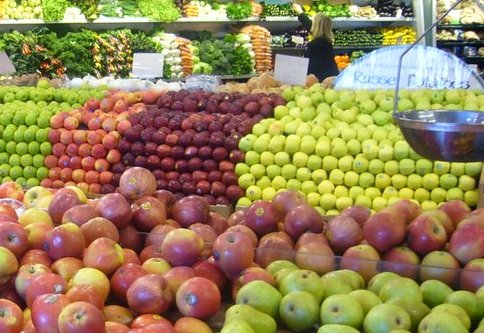
\includegraphics[width=\paperwidth,height=\paperheight]{../Art/Apples_supermarket_cropped.jpg}
}
\begin{frame}[plain]
\end{frame}
}


\centeredlargetext{black}{white}{
Excludable Goods
}


\centeredlargetext{black}{white}{
Public Goods
}


\centeredlargetext{black}{white}{
Common Property\\
Resources
}

\centeredlargetext{black}{white}{
Open Access\\
Resources
}


\centeredlargetext{white}{black}{
The Coordination\\
Problem
}


{
\setbeamertemplate{navigation symbols}{}
\setbeamertemplate{background canvas}{
  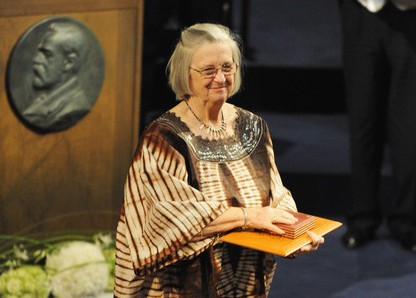
\includegraphics[width=\paperwidth,height=\paperheight]{../Art/ElinorOstromNobelPrizeCeremony2009.jpg}
}
\begin{frame}[plain]
\end{frame}
}


\begin{frame}
\frametitle{Governance}
\Huge
\begin{itemize}
\item Fisheries
\pause
\item Forests
\pause
\item Irrigation channels
\pause
\item Underground Water Basins
\end{itemize}
\end{frame}


\begin{frame}
\frametitle{Management of Common Pool Resources}
\Large
\begin{itemize}
\item Mountain Forest/Grazing in \textbf{Switzerland}, \textbf{500} years
\pause
\item Mountain Forest/Grazing in \textbf{Japan}, \textbf{400} years
\pause
\item Irrigation Systems in \textbf{Spain}, \textbf{1,000} years
\pause
\item Irrigation Systems in the \textbf{Philippines}, \textbf{500} years
\pause
\item Water Basins in \textbf{California}, \textbf{50} years
\end{itemize}
\end{frame}


\section{Practices}

\begin{frame}
\frametitle{Governance}
\Huge
\begin{itemize}
\item Benevolent Dictator
\pause
\item Community Concensus
\end{itemize}
\end{frame}


{
\setbeamertemplate{navigation symbols}{}
\setbeamertemplate{background canvas}{
  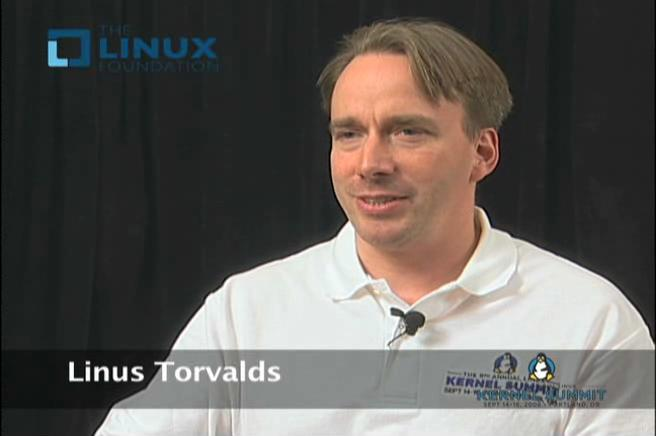
\includegraphics[width=\textwidth,height=\paperheight]{../Art/Linus_Torvalds_lks08.jpg}
}
\begin{frame}[plain]
\end{frame}
}



\centeredlargetext{black}{white}{
Free\\
Rider
}


{
\setbeamertemplate{navigation symbols}{}
\setbeamertemplate{background canvas}{
  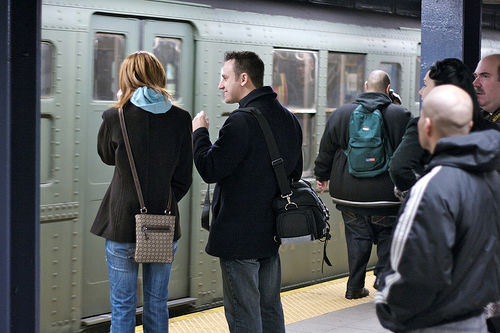
\includegraphics[width=\paperwidth,height=\paperheight]{../Art/2150546585_b3389ea99e_smaller.jpg}
}
\begin{frame}[plain]
\end{frame}
}


\centeredlargetext{black}{white}{
The Problem of\\
Commitment
}


\centeredlargetext{black}{white}{
\emph{``Nobody wants\\
to be a sucker''}
}


\centeredlargetext{black}{white}{
Conditional\\
Compliance
}


{
\begin{frame}[plain]
\Huge
\center
\begin{center}
The Problem of\\
Mutual Monitoring
\end{center}
\end{frame}
}


{
\setbeamertemplate{navigation symbols}{}
\begin{frame}
  \frametitle{Quality Control Dashboard}
  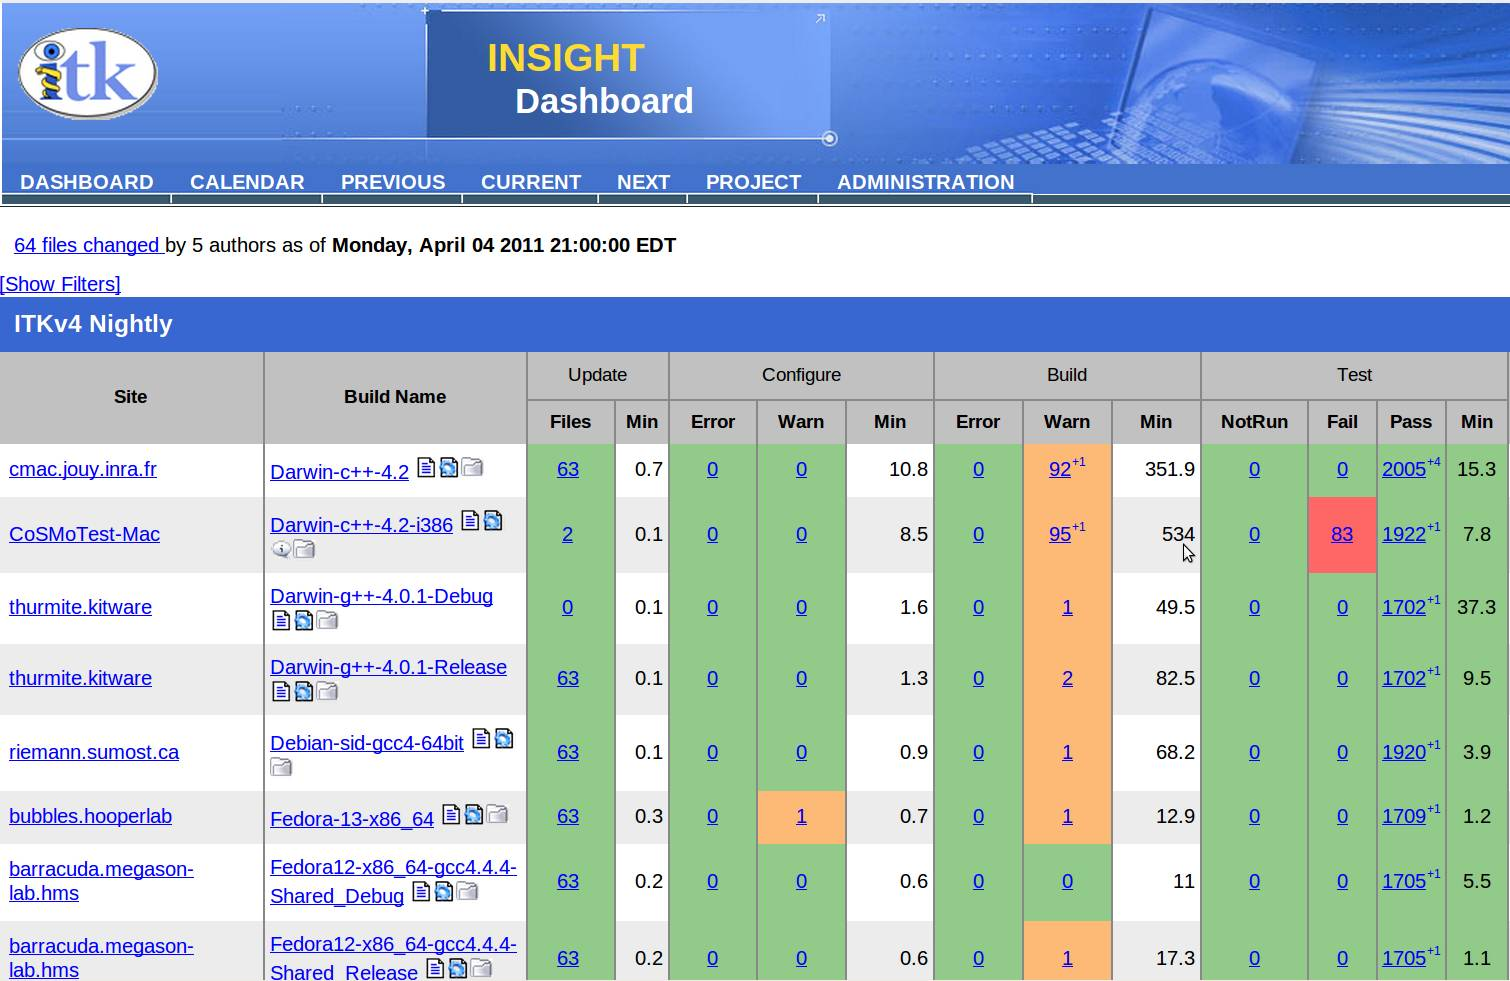
\includegraphics[width=\textwidth,height=\paperheight]{../Art/ITKDashboardScreenShot.jpg}
\end{frame}
}


\centeredlargetext{black}{white}{
Free Flow of\\
Information
}


\begin{frame}
\frametitle{Bug/Issue Trackers}
\Huge
\begin{itemize}
\item Two-Way Communication
\pause
\item Developes and Community exchange information
\pause
\item History of Bugs / Actions
\end{itemize}
\end{frame}


\begin{frame}
\frametitle{Bug/Issue Trackers}
\Huge
\begin{itemize}
\item Bug Fixing
\pause
\item Project Coordination
\pause
\item Avoid Duplication of Effort
\pause
\item Project Planning
\end{itemize}
\end{frame}


\begin{frame}
\frametitle{The Secret Life of Bugs}
\Huge
\begin{center}
Coverity\\
\bigskip
Report\footnote{\url{http://scan.coverity.com/all-projects.html}}
\end{center}
\end{frame}


\begin{frame}
\frametitle{The Coverity Report}
\Huge
\begin{center}
\textbf{10 Defects} per\\
\bigskip
\textbf{1000 Lines} of code\footnote{Average of the Industry}
\end{center}
\end{frame}

\begin{frame}
\frametitle{The Secret Life of Bugs}
\Huge
\begin{center}
Firefox\\
\bigskip
0.162 defects per 1000 lines\footnote{\url{http://scan.coverity.com/all-projects.html}}
\end{center}
\end{frame}


\begin{frame}
\frametitle{The Secret Life of Bugs}
\Huge
\begin{center}
Linux Kernel 2.6\\
\bigskip
0.127 defects per 1000 lines\footnote{\url{http://scan.coverity.com/all-projects.html}}

\end{center}
\end{frame}


\begin{frame}
\frametitle{The Secret Life of Bugs}
\Huge
\begin{center}
KDE\\
\bigskip
0.019 defects per 1000 lines\footnote{\url{http://scan.coverity.com/all-projects.html}}
\end{center}
\end{frame}


\begin{frame}
\frametitle{The Secret Life of Bugs}
\Huge
When coverity reported\\
\pause
985 bugs\\
\pause
in the Linux Kernel (2004)\\
\end{frame}


\begin{frame}
\frametitle{The Secret Life of Bugs}
\Huge
They were all fixed\\
\pause
in \textbf{six months}\\
\end{frame}


\begin{frame}
\frametitle{The Secret Life of Bugs}
\Huge
Most Bugs are introduced\\
\bigskip
\pause
\textbf{WHILE}\\
\bigskip
trying to fix other bugs
\end{frame}


{
\setbeamertemplate{navigation symbols}{}
\begin{frame}
  \frametitle{Code Review}
  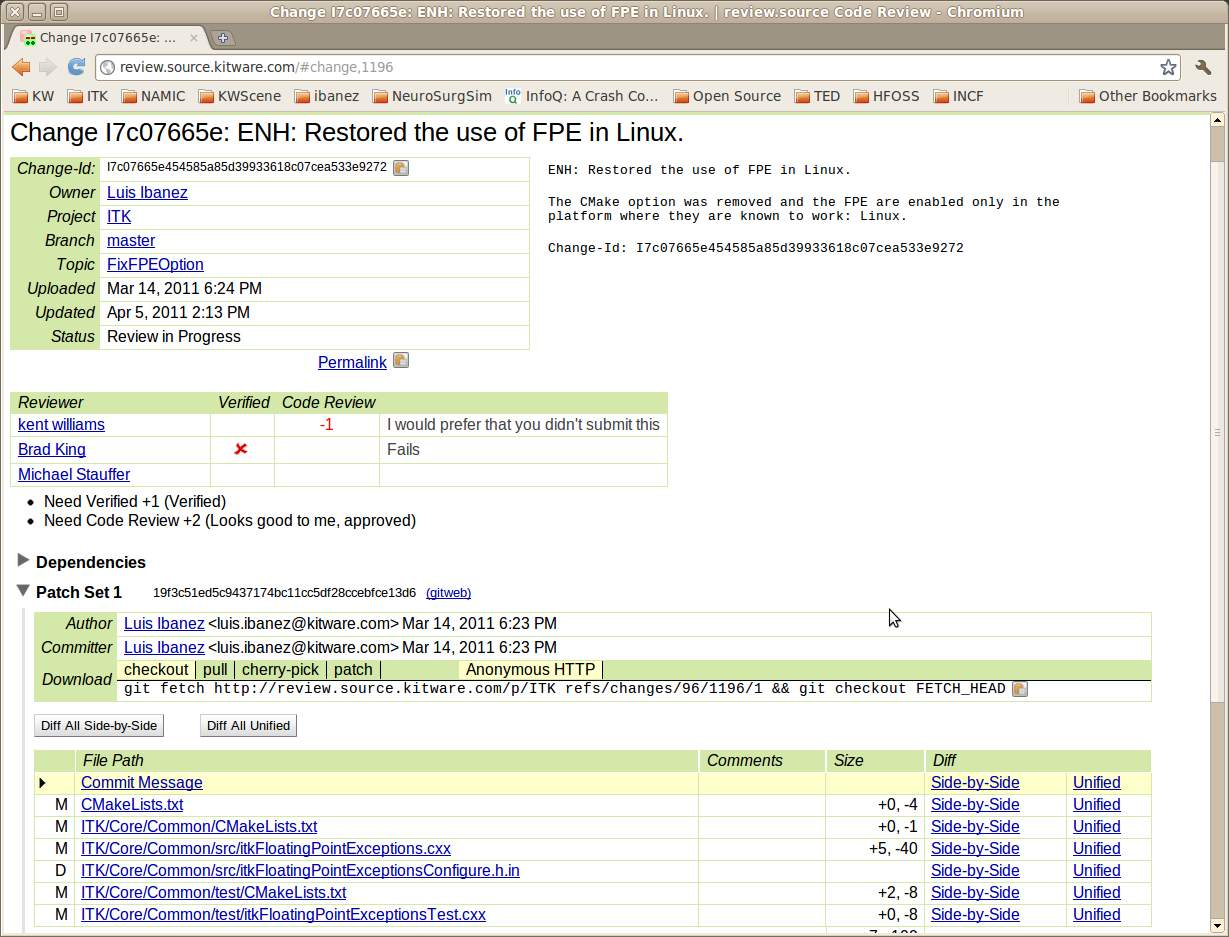
\includegraphics[width=\textwidth,height=\paperheight]{../Art/ITKGerritScreenShot.jpg}
\end{frame}
}


\begin{frame}
\frametitle{The Secret Life of Bugs}
\Huge
Maintainability
\end{frame}


\centeredlargetext{black}{white}{
Software that\\
``just works''\\
is not enough\\
}


\centeredlargetext{black}{white}{
Code is intended\\
for Humans
}


\centeredlargetext{black}{white}{
Smart Developers\\
\pause
vs.\\
Professional Developers\\
}


\centeredlargetext{black}{white}{
Cost of Ownership
}


{
\setbeamertemplate{navigation symbols}{}
\setbeamertemplate{background canvas}{
  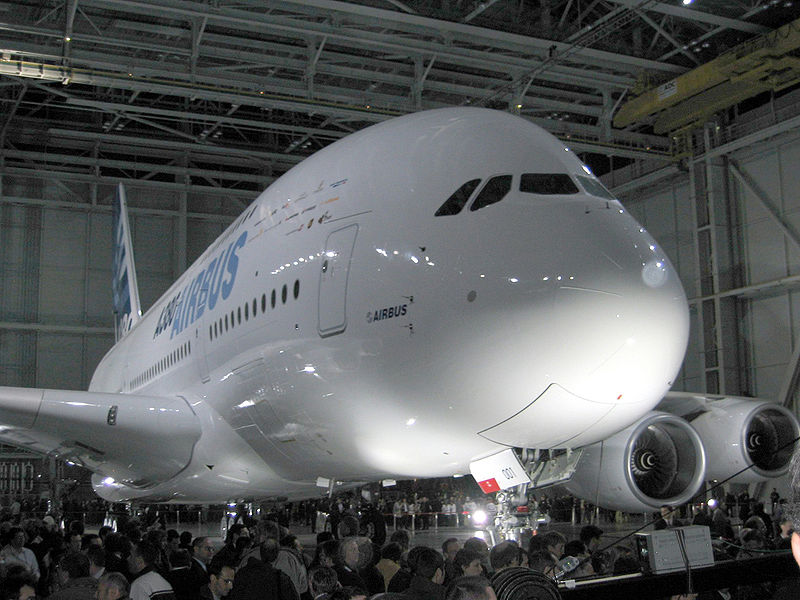
\includegraphics[width=\paperwidth,height=\paperheight]{../Art/800px-A380_Reveal_1.jpg}
}
\begin{frame}[plain]
\end{frame}
}


{
\setbeamertemplate{navigation symbols}{}
\setbeamertemplate{background canvas}{
  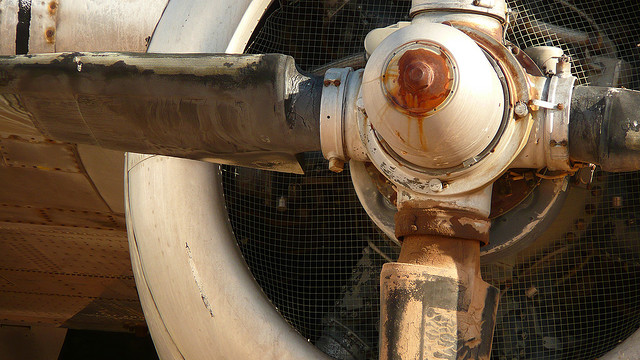
\includegraphics[width=\paperwidth,height=\paperheight]{../Art/2173190174_b2b2d03f21_z.jpg}
}
\begin{frame}[plain]
\end{frame}
}


\centeredlargetext{black}{white}{
Take care of your bugs\\
every day\ldots
}


\begin{frame}
\frametitle{The Secret Life of Bugs}
\Huge
If not fixed in 5 days\ldots
\end{frame}


\begin{frame}
\frametitle{Days to Fix a Bug in an Open Source Project (ITK)}
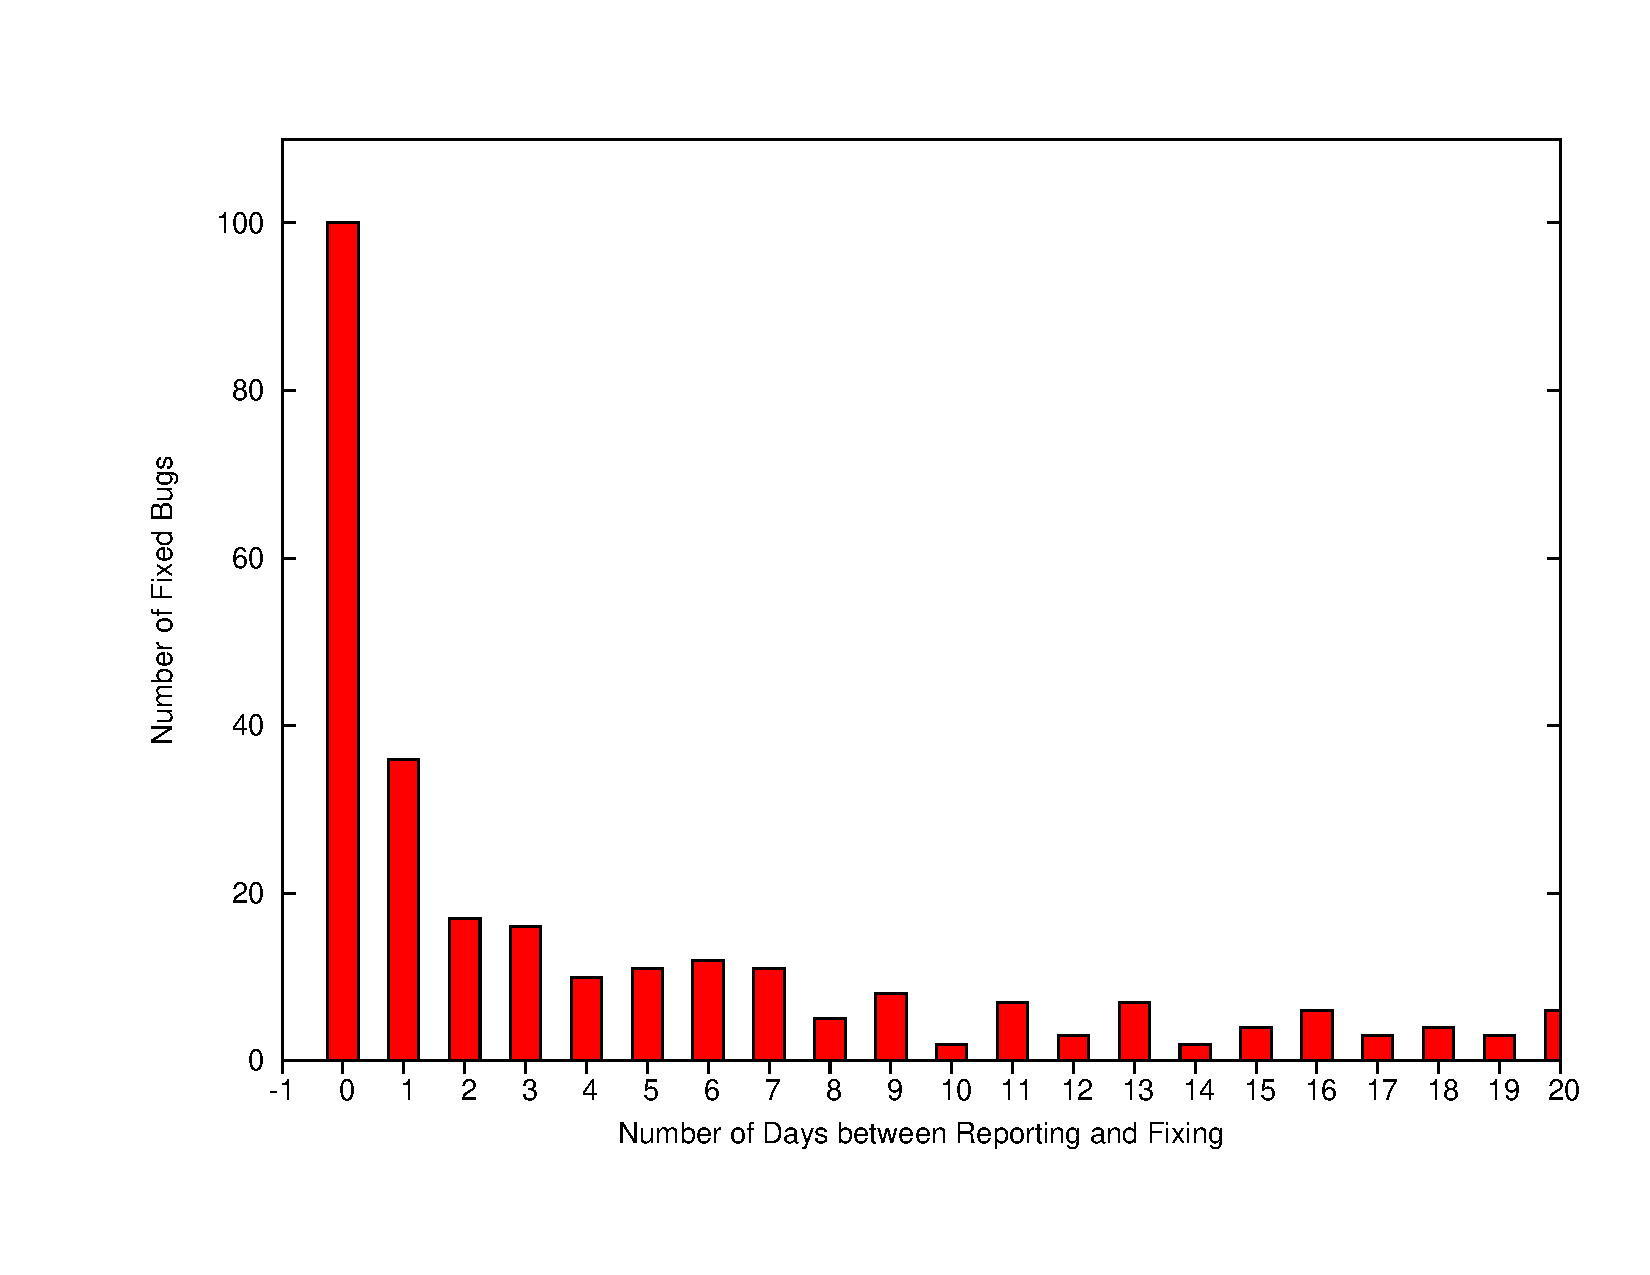
\includegraphics[width=0.9\textwidth,height=0.9\paperheight]{../Art/ITKBugFixesScheduleHistogramPlot.pdf}
\end{frame}


\begin{frame}
\frametitle{Days to Fix a Bug in an Open Source Project (ITK)}
\Huge
\begin{itemize}
\item 11\% the same day
\pause
\item 22\% in 1 week
\pause
\item 27\% in 2 week
\pause
\item 30\% in 1 month
\pause
\item Longest time 2,589 days
\end{itemize}
\end{frame}


{
\setbeamertemplate{navigation symbols}{}
\begin{frame}
\frametitle{Bug/Issue Tracker}
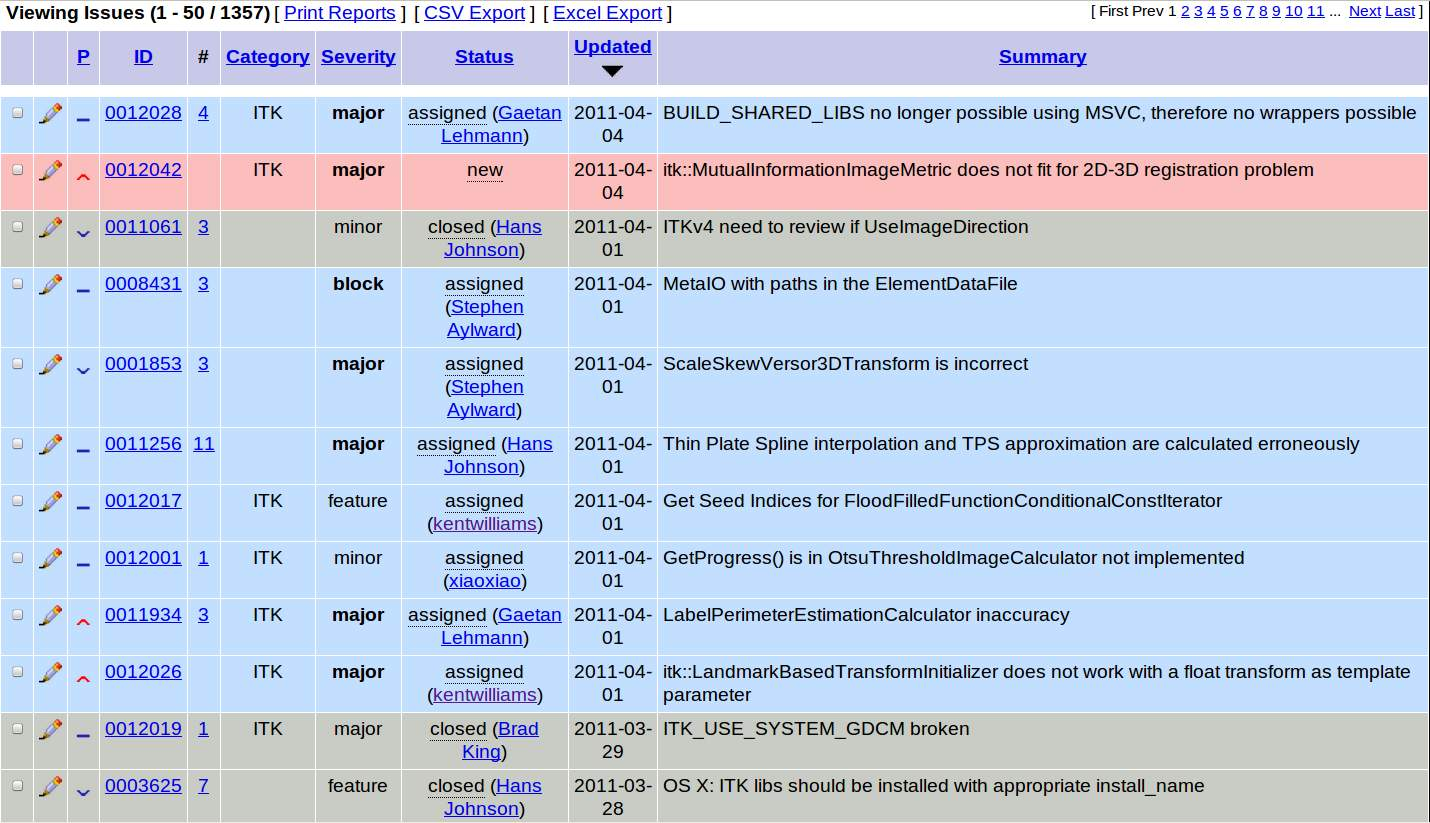
\includegraphics[width=0.9\textwidth,height=0.9\paperheight]{../Art/ITKMANTISScreenShot.jpg}
\end{frame}
}


{
\setbeamertemplate{navigation symbols}{}
\begin{frame}
\frametitle{Wikis}
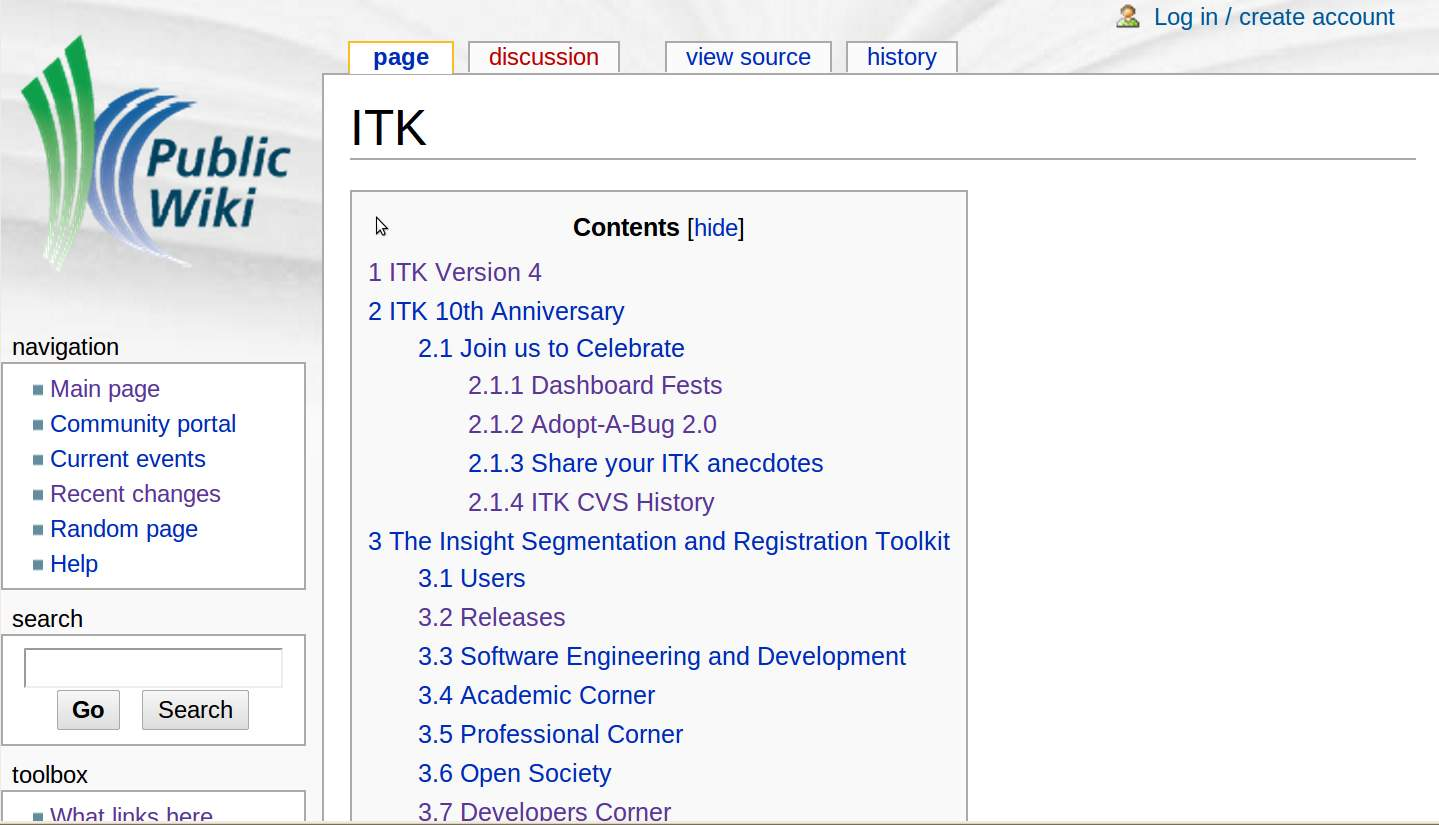
\includegraphics[width=0.9\textwidth,height=0.9\paperheight]{../Art/ITKWikiScreenShot.jpg}
\end{frame}
}




\begin{frame}
\frametitle{Code Repositories}
\Huge
\begin{itemize}
\item Backup
\pause
\item History of Changes
\pause
\item Collaboration Platform
\end{itemize}
\end{frame}


\begin{frame}
\frametitle{Code Repositories}
\Huge
\begin{itemize}
\item Who ?
\pause
\item What ?
\pause
\item When ?
\pause
\item \textbf{Why} ?
\end{itemize}
\end{frame}


\begin{frame}
\frametitle{Code Repositories}
\Huge
Typical Choices
\begin{itemize}
\item CVS
\pause
\item SVN
\pause
\item Git
\pause
\item Mercurial
\end{itemize}
\end{frame}


\begin{frame}
\frametitle{Code Repositories - Gitorius}
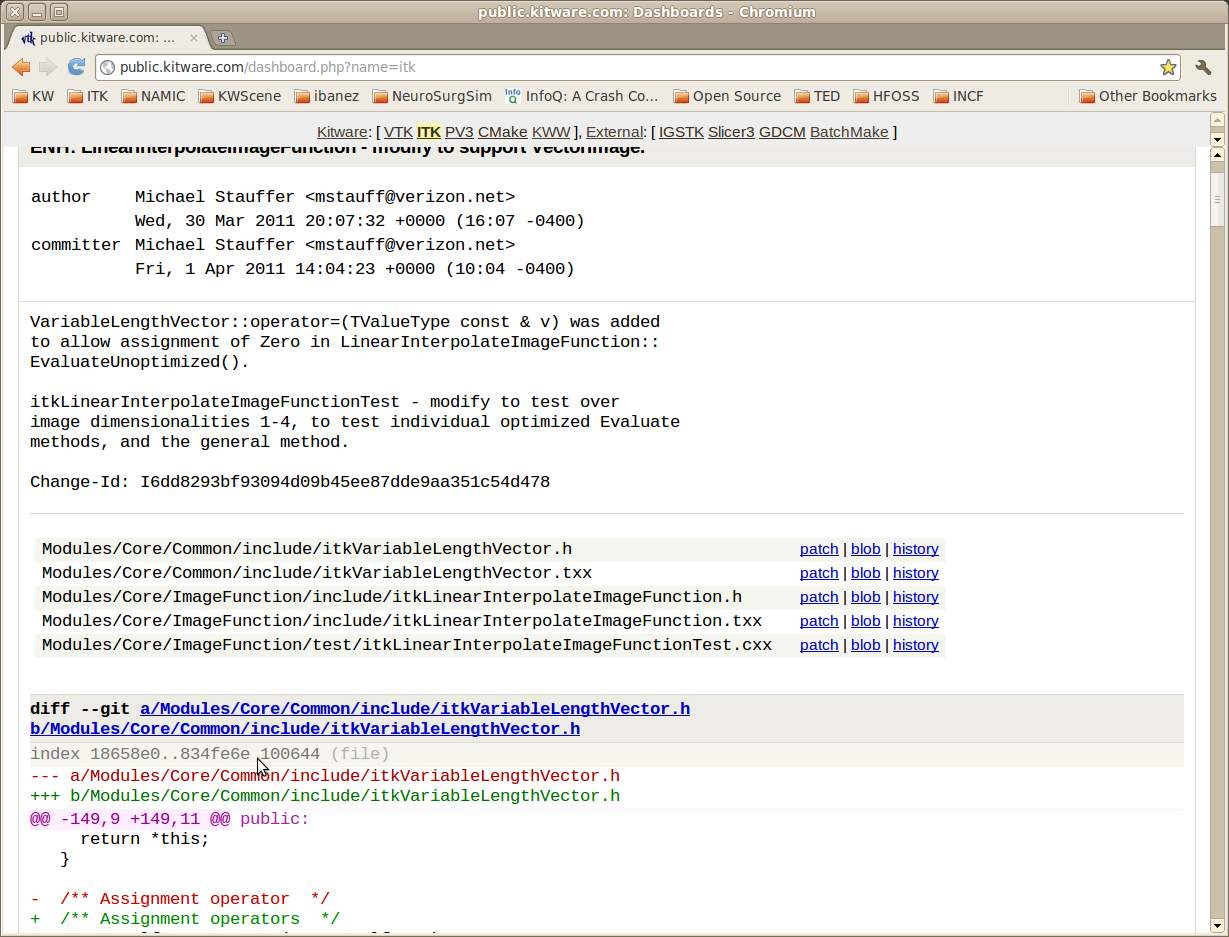
\includegraphics[width=0.9\textwidth,height=0.9\paperheight]{../Art/ITKGitScreenShot.jpg}
\end{frame}


\begin{frame}
\frametitle{Code Repositories - Github}
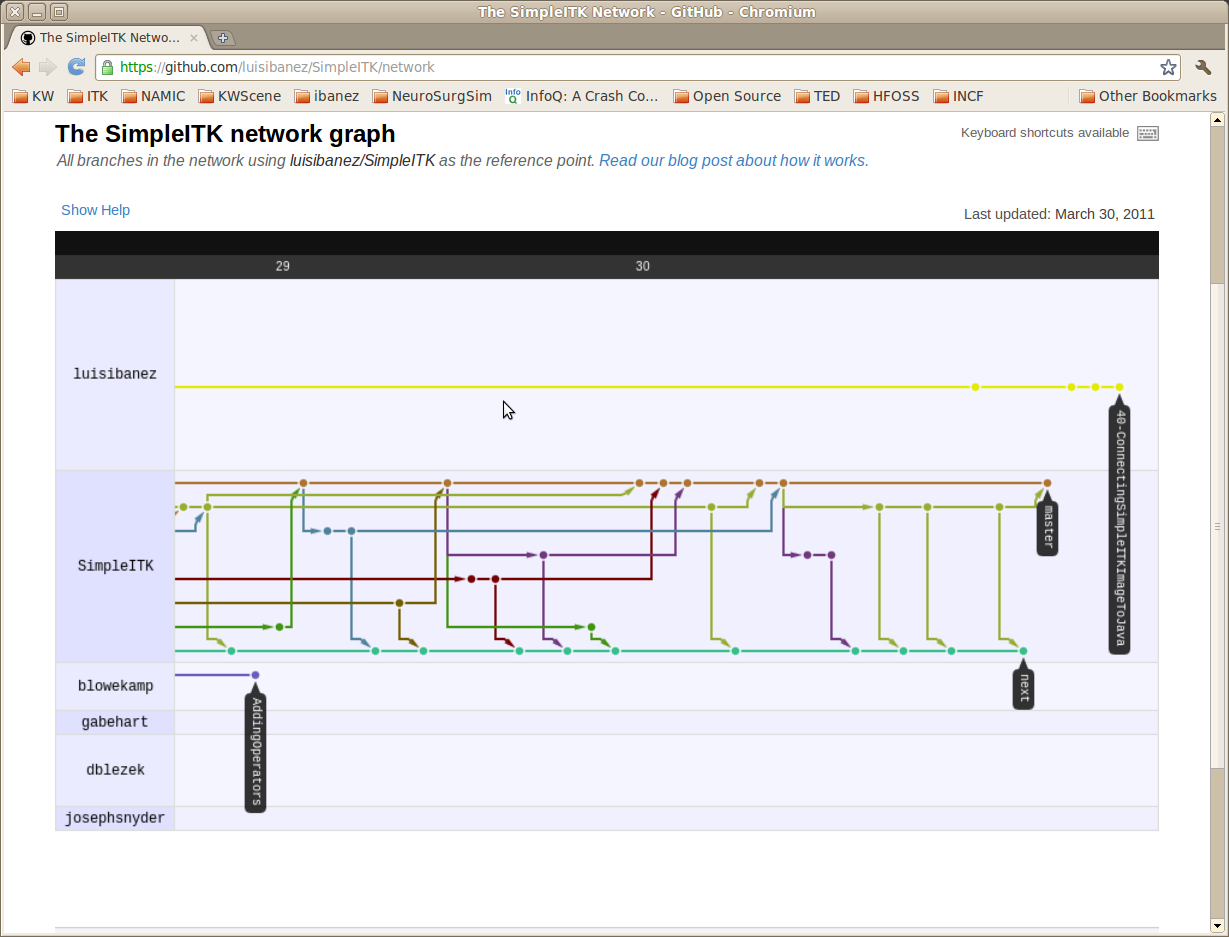
\includegraphics[width=0.9\textwidth,height=0.9\paperheight]{../Art/SimpleITKGithubScreenShot.jpg}
\end{frame}


\begin{frame}
\frametitle{Distributed Code Repositories}
\Huge
\begin{itemize}
\item Branching and Merging
\pause
\item Peripherial Development
\pause
\item Clean Releases
\end{itemize}
\end{frame}


\begin{frame}
\frametitle{Real Open Source - Best Practices}
\Huge
\begin{itemize}
\item Open from day zero
\pause
\item OSI-approved license
\pause
\item Release Early Release Often
\end{itemize}
\end{frame}


\part{Why Open Source ?}

\centeredlargetext{black}{white}{
To be in control\\
of your Destiny...
}


\centeredlargetext{black}{white}{
Indirect\\
Appropriation
}


\centeredlargetext{black}{white}{
Guarrantee\\
Longevity
}


\centeredlargetext{black}{white}{
Support
}


\centeredlargetext{black}{white}{
Competition
}


\begin{frame}[plain]
\fontsize{30pt}{30pt}\selectfont
\center
\begin{quote}
Finished products\\
are for decadent minds
\end{quote}
\bigskip
\fontsize{18pt}{18pt}\selectfont
\begin{flushright}
Isaac Asimov\\
``The Foundation''
\end{flushright}
\end{frame}


\begin{frame}
\frametitle{Credits}
\begin{itemize}
\item \url{http://opensource.org/files/osi_standard_logo.png}
\item \url{http://www.flickr.com/photos/lifeontheedge/2672465894}
\item \url{http://www.flickr.com/photos/hortulus_aptus/4293485922}
\item \url{http://en.wikipedia.org/wiki/File:Iceberg_Antarctica.jpg}
\item \url{http://en.wikipedia.org/wiki/File:Iceberg.jpg}
\item \url{http://en.wikipedia.org/wiki/File:Hyundai_car_assembly_line.jpg}
\item \url{http://www.flickr.com/photos/spencer77/4924182750}
\item \url{http://www.zimbio.com/photos/Elinor+Ostrom/Nobel+Prize+Award+Ceremony+2009/quiD3nGLq-e}
\end{itemize}
\end{frame}


\begin{frame}
\frametitle{Credits}
\begin{itemize}
\item \url{http://www.flickr.com/photos/mwichary/2150546585}
\item \url{http://commons.wikimedia.org/wiki/File:Linus_Torvalds_lks08.jpg}
\item \url{http://en.wikipedia.org/wiki/File:Apples_supermarket.jpg}
\item \url{http://www.flickr.com/photos/amagill/3366720659}
\item \url{http://www.flickr.com/photos/vectorportal/4047547668/}
\item \url{http://en.wikipedia.org/wiki/File:A380_Reveal_1.jpg}
\item \url{http://www.flickr.com/photos/arollinger/2173190174}
\end{itemize}
\end{frame}


\end{document}
